\documentclass[10pt]{article}

\usepackage[a4paper,margin=20mm]{geometry}
\usepackage[T1]{fontenc}
\usepackage[utf8]{inputenc}
\usepackage{amsmath,amssymb}
\usepackage{array,booktabs}
\usepackage{graphicx}
\usepackage{float}
\usepackage{xcolor}
\usepackage{tikz}
\usetikzlibrary{arrows.meta,positioning,shapes.geometric,fit,backgrounds,calc}
\usepackage[numbers,sort&compress]{natbib}
\usepackage[colorlinks=true,linkcolor=blue!55!black,citecolor=blue!55!black,urlcolor=blue!55!black]{hyperref}
\usepackage{url}

\graphicspath{{figures/}}
\setlength{\parindent}{0pt}
\setlength{\parskip}{5pt}
\setlength{\tabcolsep}{4.5pt}
\renewcommand{\arraystretch}{1.12}

\definecolor{fifo}{HTML}{4C78A8}
\definecolor{reservoir}{HTML}{F58518}
\definecolor{irgreen}{HTML}{54A24B}
\definecolor{danger}{HTML}{E45756}
\definecolor{lightblue}{HTML}{DBE9F6}
\definecolor{lightorange}{HTML}{FCE5CC}
\definecolor{lightgreen}{HTML}{DCEFD9}

\newcommand{\fifo}{\textsc{FIFO}}
\newcommand{\res}{\textsc{Reservoir}}
\newcommand{\ir}{\textsc{IR}}
\newcommand{\pct}[1]{#1\%}
\newcommand{\pp}{\,pp}

\title{\textbf{Goal-Stratified Reservoir Replay and Actor-Only Imagined Rehearsal\\in Sequential RLScape}\\[3pt]
\large A three-task, 1.5-million-step checkpoint study}
\author{Steven Davenport\\Continual Reinforcement Learning Research Notes}
\date{Experiment completed August 2026; report generated 8 August 2026}

\begin{document}
\maketitle

\begin{abstract}
We study sequential goal learning in RLScape using a goal-conditioned DreamerV3 agent. One agent encounters \emph{kill goblin}, \emph{bury bones}, and \emph{chop logs} for 500k environment steps each. We compare the original 200k-capacity global FIFO replay workflow against a persistent, goal-stratified reservoir containing up to 1,000 complete episodes per goal. At six pinned checkpoints, every goal encountered so far is evaluated with a frozen actor and with actor-only imagined rehearsal (IR), under both sampled and deterministic action selection. The reservoir run completed without a crash in approximately 82 hours and produced 3,600 evaluation episodes. Reservoir replay was demonstrably functional: during the final task it simultaneously recovered earlier goals while learning the current goal, and at 1.25M steps its worst sampled-policy task reached \pct{49} versus \pct{8} for FIFO. However, it did not stabilize the learner. By 1.5M steps all reservoir goals had collapsed to at most \pct{16} frozen success, and mean frozen success was \pct{9.7}, compared with \pct{61.7} for FIFO. Ungated actor IR was similarly conditional. Across all reservoir cells it reduced sampled success by 6.5 percentage points on average, but at the final damaged checkpoint it improved mean success by 5.6 points and improved kill-goblin by 12 points. These results reject the simple hypothesis that balanced reservoir replay alone solves retention. They support a narrower conclusion: retained old data and test-time actor adaptation can recover behavior, but the world-model/value/policy system remains dynamically unstable and IR should be gated or otherwise regularized.
\end{abstract}

\section{Research question and contribution}

The long-term research direction is continual reinforcement learning over an RLScape task landscape: train on goals $A\rightarrow B\rightarrow C\rightarrow\cdots$, repeatedly evaluate all previous goals, and measure both forgetting and transfer speed relative to a non-IR baseline. The immediate question was narrower. The preceding FIFO experiment suggested that later phases remove most early-task data, potentially weakening the goal-conditioned reward model and value function that IR relies on. We therefore asked:

\begin{enumerate}
  \item Does goal-stratified reservoir replay preserve earlier goal competence better than global FIFO replay?
  \item Does a retained multi-goal world model and critic make actor-only IR useful at evaluation time?
  \item Can the system train continuously for 1.5M steps with research-grade checkpoint and evaluation integrity?
\end{enumerate}

The experiment contributes a fully persisted three-goal sequential run, six immutable training checkpoints, 24 paired frozen/IR evaluation units, two action-selection modes, and a direct comparison to the previous FIFO run. It is an exploratory, single-seed systems experiment rather than a population-level statistical claim.

\section{Experimental design}

\subsection{Task sequence}

The agent trained on three goals in a fixed curriculum:

\begin{figure}[H]
\centering
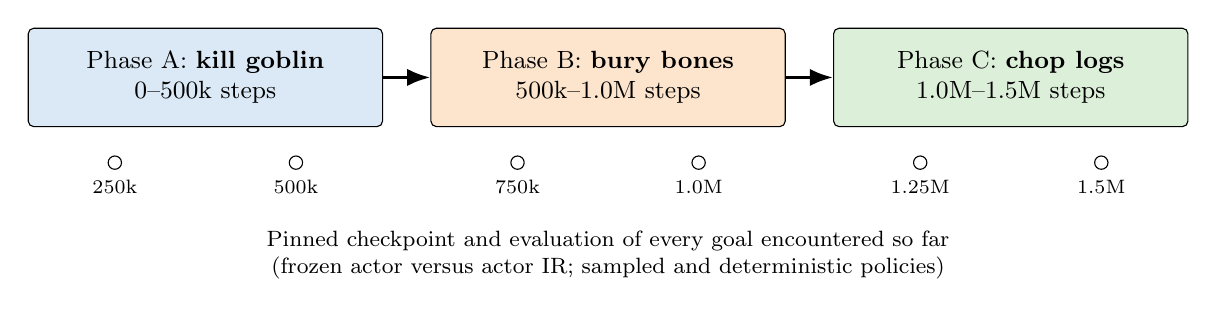
\begin{tikzpicture}[
  >=Latex,
  phase/.style={draw,rounded corners=2pt,minimum width=4.5cm,minimum height=1.25cm,align=center,font=\small},
  eval/.style={draw,circle,fill=white,inner sep=1.7pt,font=\scriptsize},
  arrow/.style={->,very thick}
]
\node[phase,fill=lightblue] (a) {Phase A: \textbf{kill goblin}\\0--500k steps};
\node[phase,fill=lightorange,right=6mm of a] (b) {Phase B: \textbf{bury bones}\\500k--1.0M steps};
\node[phase,fill=lightgreen,right=6mm of b] (c) {Phase C: \textbf{chop logs}\\1.0M--1.5M steps};
\draw[arrow] (a) -- (b);
\draw[arrow] (b) -- (c);
\foreach \x/\lab in {-1.15/250k,1.15/500k} {\node[eval] at ($(a.south)+(\x,-.45)$) {}; \node[below,font=\scriptsize] at ($(a.south)+(\x,-.55)$) {\lab};}
\foreach \x/\lab in {-1.15/750k,1.15/1.0M} {\node[eval] at ($(b.south)+(\x,-.45)$) {}; \node[below,font=\scriptsize] at ($(b.south)+(\x,-.55)$) {\lab};}
\foreach \x/\lab in {-1.15/1.25M,1.15/1.5M} {\node[eval] at ($(c.south)+(\x,-.45)$) {}; \node[below,font=\scriptsize] at ($(c.south)+(\x,-.55)$) {\lab};}
\node[below=12mm of b,font=\footnotesize,align=center] {Pinned checkpoint and evaluation of every goal encountered so far\\(frozen actor versus actor IR; sampled and deterministic policies)};
\end{tikzpicture}
\caption{Sequential curriculum and evaluation ladder. There is no return phase in this experiment. The checkpoints permit later ablations without retraining the full curriculum.}
\label{fig:timeline}
\end{figure}

Each episode was capped at 200 actions and used sparse binary task-completion reward. The action interface was a flat $28\times18$ click grid, giving 504 discrete click locations. This was intentionally held fixed between replay conditions so the comparison isolates replay, not environment design.

\subsection{Agent and training configuration}

The implementation uses DreamerV3 \citep{hafner2023dreamerv3} with the repository's ``50m'' preset. The observed trainable parameter count was approximately 77.3M; the preset name is therefore a configuration label, not the measured parameter total. The recurrent state-space model (RSSM) uses a deterministic state of width 4,096 and a $32\times32$ categorical stochastic state. Training used batches of 8 sequences, sequence length 32, imagination horizon 15, training ratio 32, and bfloat16 computation on a 24,GB GPU.

Let $o_t$ be the image, $a_t$ the click action, and $s_t=(h_t,z_t)$ the Dreamer latent state. The goal-agnostic dynamics are
\begin{align}
 h_t &= f_\phi(h_{t-1},z_{t-1},a_{t-1}),\\
 z_t &\sim q_\phi(z_t\mid h_t,e_\phi(o_t)) \quad\text{during representation learning},\\
 z_t &\sim p_\phi(z_t\mid h_t) \quad\text{during imagination}.
\end{align}
Five RLScape goals are represented by a five-dimensional one-hot vector $g_t$, although only three goal IDs occur in this experiment. The behavior feature is
\begin{equation}
 x_t=[h_t;z_t;g_t].
\end{equation}
The reward, continuation, actor, value, and slow-value heads consume $x_t$:
\begin{align}
 \hat r_t&\sim p_\phi(r_t\mid h_t,z_t,g_t), &
 \hat c_t&\sim p_\phi(c_t\mid h_t,z_t,g_t),\\
 a_t&\sim\pi_\theta(a_t\mid h_t,z_t,g_t), &
 v_\psi&=v_\psi(h_t,z_t,g_t).
\end{align}
The RSSM transition and visual representation remain goal-agnostic. Thus the shared latent should model what is happening on screen, while the heads interpret that state under the requested goal.

\begin{figure}[H]
\centering
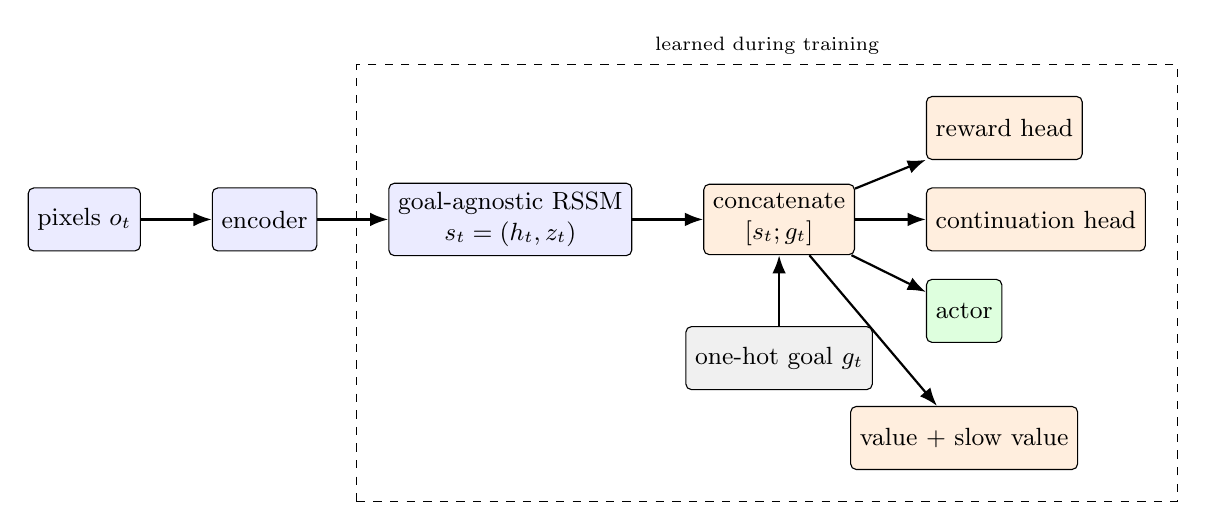
\begin{tikzpicture}[
  >=Latex,node distance=6mm and 9mm,
  box/.style={draw,rounded corners=2pt,minimum height=8mm,align=center,font=\small},
  frozen/.style={box,fill=blue!8},
  conditioned/.style={box,fill=orange!13},
  trainable/.style={box,fill=green!13},
  flow/.style={->,thick}
]
\node[frozen] (obs) {pixels $o_t$};
\node[frozen,right=of obs] (enc) {encoder};
\node[frozen,right=of enc] (rssm) {goal-agnostic RSSM\\$s_t=(h_t,z_t)$};
\node[conditioned,right=of rssm] (join) {concatenate\\$[s_t;g_t]$};
\node[conditioned,above right=3mm and 9mm of join] (rew) {reward head};
\node[conditioned,right=9mm of join] (cont) {continuation head};
\node[trainable,below right=3mm and 9mm of join] (actor) {actor};
\node[conditioned,below=8mm of actor] (value) {value + slow value};
\node[box,below=9mm of join,fill=gray!12] (goal) {one-hot goal $g_t$};
\draw[flow] (obs)--(enc); \draw[flow] (enc)--(rssm); \draw[flow] (rssm)--(join);
\draw[flow] (goal)--(join); \draw[flow] (join)--(rew); \draw[flow] (join)--(cont);
\draw[flow] (join)--(actor); \draw[flow] (join)--(value);
\node[draw,dashed,fit=(rssm)(join)(rew)(cont)(actor)(value),inner sep=4mm,label={[font=\scriptsize]above:learned during training}] {};
\end{tikzpicture}
\caption{Goal-conditioning architecture. During evaluation-time IR, only the actor parameters (green) are updated; the world model, reward/continuation heads, and critic/value functions are frozen.}
\label{fig:architecture}
\end{figure}

\subsection{Replay conditions}

\paragraph{FIFO baseline.}
The comparison run used the original global replay with capacity 200,000 sequence starts. Once full, newly collected experience evicts the oldest experience regardless of goal. Uniform training batches therefore increasingly reflect the current phase.

\paragraph{Goal-stratified episode reservoir.}
The new replay stores at most $M_g=1{,}000$ complete episodes independently for each represented goal, for a total capacity of 3,000 episodes. Within goal $g$, the $n_g$th observed episode is processed by Algorithm R \citep{vitter1985reservoir}:
\begin{equation}
 \Pr(\text{admit episode }n_g)=\min\left(1,\frac{M_g}{n_g}\right).
\end{equation}
If admitted after the group is full, it uniformly replaces one of the $M_g$ resident episodes. Consequently every historical episode for a goal has equal probability $M_g/n_g$ of residing in that goal's reservoir. Training samples a represented goal uniformly, an episode uniformly within that goal, and then a random sequence start. Short fragments are concatenated with explicit \texttt{is\_first} boundaries so the recurrent state resets correctly.

\begin{figure}[H]
\centering
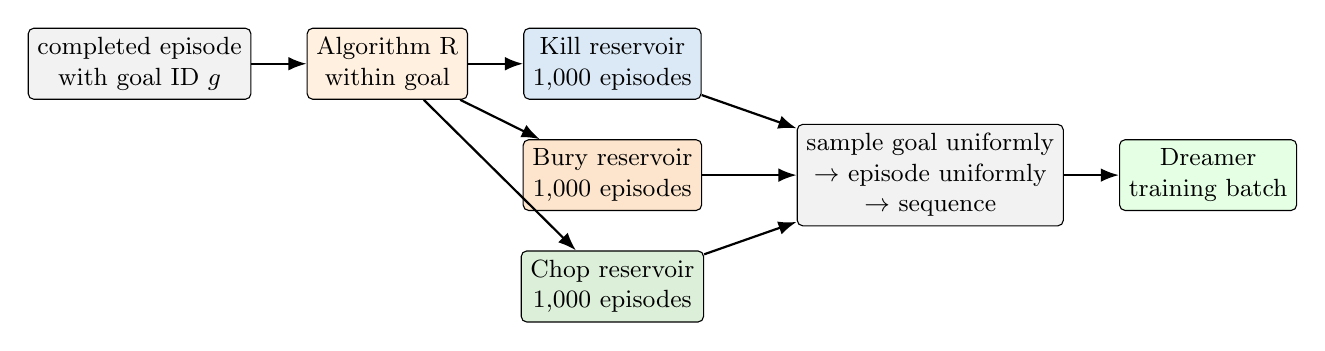
\begin{tikzpicture}[
  >=Latex,node distance=5mm and 7mm,font=\small,
  bx/.style={draw,rounded corners=2pt,minimum height=8mm,align=center},
  ar/.style={->,thick}
]
\node[bx,fill=gray!10] (stream) {completed episode\\with goal ID $g$};
\node[bx,fill=orange!12,right=of stream] (alg) {Algorithm R\\within goal};
\node[bx,fill=lightblue,right=of alg] (r1) {Kill reservoir\\1,000 episodes};
\node[bx,fill=lightorange,below=of r1] (r2) {Bury reservoir\\1,000 episodes};
\node[bx,fill=lightgreen,below=of r2] (r3) {Chop reservoir\\1,000 episodes};
\node[bx,fill=gray!10,right=12mm of r2] (sample) {sample goal uniformly\\$\rightarrow$ episode uniformly\\$\rightarrow$ sequence};
\node[bx,fill=green!10,right=of sample] (batch) {Dreamer\\training batch};
\draw[ar] (stream)--(alg);
\draw[ar] (alg)--(r1); \draw[ar] (alg)--(r2); \draw[ar] (alg)--(r3);
\draw[ar] (r1)--(sample); \draw[ar] (r2)--(sample); \draw[ar] (r3)--(sample);
\draw[ar] (sample)--(batch);
\end{tikzpicture}
\caption{Goal-stratified episode reservoir. Statistical retention is uniform over the episode stream within each goal; optimization sampling is balanced across represented goals.}
\label{fig:reservoir}
\end{figure}

This balance changes the effective emphasis on new data. The global training ratio remains 32, but the expected share of updates drawn from the current goal is 1, $1/2$, and $1/3$ in phases A, B, and C. In this limited sense, current-goal exposure is approximately 32, 16, and 10.7 replayed samples per environment step. This is a plausible source of slower acquisition or instability and is important when interpreting the comparison.

\subsection{Evaluation-time imagined rehearsal}

IR performs temporary test-time optimization of the actor from the agent's current latent state. For each environment action, the evaluator draws $N=128$ posterior latent samples, imagines $H=6$ steps under the frozen world model, and takes one actor gradient update with learning rate $4\times10^{-5}$. The objective is the Dreamer actor objective: increase imagined, critic-estimated return while retaining the configured entropy bonus $\eta=3\times10^{-4}$,
\begin{equation}
 \theta' \leftarrow \theta-\alpha\nabla_\theta
 \left[-\mathbb E_{\hat\tau\sim p_\phi,\pi_\theta}
 \left(\widehat A_\psi(\hat\tau)+\eta\,\mathcal H[\pi_\theta(\cdot\mid \hat s,g)]\right)\right].
\end{equation}
The precise implementation uses the repository's normalized imagined-advantage actor loss. The world model, reward/continuation models, critic, and slow critic are frozen. Actor updates accumulate within an episode, are discarded at the episode boundary, and never alter the saved training checkpoint. There is no confidence, entropy, or value-based gate: IR runs at every action from the first action ($k=0$).

Conceptually, IR asks whether the retained model and critic contain enough goal-specific knowledge to repair a locally damaged actor without collecting gradient updates from the real reward stream. It is not hindsight relabeling \citep{andrychowicz2017her}: replay goals and rewards are not relabeled.

\subsection{Evaluation protocol and integrity}

At 250k-step intervals, every goal encountered by that point was evaluated. For each checkpoint--goal cell we ran:
\begin{itemize}
  \item 100 frozen and 100 IR episodes with sampled actions;
  \item 50 frozen and 50 IR episodes with deterministic actions.
\end{itemize}
Frozen and IR conditions used matching seed schedules and goal requests. Across 12 checkpoint--goal cells this yielded 3,600 episodes in 48 complete conditions (24 frozen/IR pairs). Requested episode counts, goal IDs, reset counts, return codes, and checkpoint parameter digests passed the evaluator's integrity checks. Because frozen and IR conditions ran in separate RLScape process lifetimes, their initial image hashes were not identical despite matching seed/goal identities. The analysis therefore treats them as seed-paired aggregate comparisons, not guaranteed pixel-identical counterfactual trajectories.

The FIFO evaluation predates a fix to the strict frame-hash pairing checker: its queue recorded failure even though individual condition summaries completed. We use the complete first attempts at checkpoints through 1.5M steps descriptively. This caveat does not affect the reservoir run's own completion status.

\section{Results}

\subsection{Execution and systems outcome}

The reservoir experiment completed all six training milestones and all 24 paired evaluation units without a training restart. Training took approximately 62.3 hours, evaluation 19.7 hours, and the full workflow approximately 82 hours. This satisfies the operational objective: a multi-day continual experiment can train, checkpoint, resume evaluation, and terminate cleanly.

At 1.5M steps the reservoir contained exactly 1,000 episodes per goal, 18,574 historical episodes had been considered for admission, and the retained episodes comprised 265,802 transitions. The latest sampling interval drew 655, 652, and 693 batches from kill, bury, and chop respectively, demonstrating near-uniform goal selection. Replay occupied 28.5,GiB of host memory and the full process 34.3,GiB, leaving 22.9,GiB available on the 62,GiB machine. Acting and training throughput were approximately 6.66 and 213 steps/s. The FIFO endpoint used 23.2,GiB for replay and 26.5,GiB for the process, with 6.92 acting steps/s and 222 training steps/s. The methods are therefore not memory-matched.

\begin{figure}[H]
\centering

\includegraphics[width=.94\linewidth]{training_success.pdf}
\caption{Training success in successive 50k-step bins. FIFO learns each active task cleanly after an initial delay. Reservoir replay reaches high success on every phase but exhibits repeated large collapses, including late in the final phase. These are behavioral training metrics, not held-out evaluation.}
\label{fig:training}
\end{figure}

Reservoir training reached rolling 100-episode peaks of \pct{99}, \pct{100}, and \pct{100} on kill, bury, and chop, proving that the architecture and action interface can solve every chosen goal. Final rolling success was only \pct{85}, \pct{54}, and \pct{16}. In the last 10k steps of each phase, success was \pct{84.2}, \pct{37.5}, and \pct{11.3}. The main failure is therefore retention/stability, not basic reachability.

\begin{figure}[H]
\centering

\includegraphics[width=.92\linewidth]{resource_footprint.pdf}
\caption{Resource use at pinned milestones. Episode capacity does not fix transition count because episode lengths vary. The 3,000-episode reservoir ended larger than the 200k-start FIFO buffer, making the comparison intentionally algorithmic rather than memory-matched.}
\label{fig:resources}
\end{figure}

\subsection{Frozen-policy checkpoint matrix}

\begin{figure}[H]
\centering

\includegraphics[width=.98\linewidth]{frozen_eval_heatmaps.pdf}
\caption{Frozen-actor success at all evaluable checkpoint--goal cells. Gray cells correspond to goals not yet introduced. The reservoir temporarily improves balanced retention but undergoes synchronized collapses at 1.0M and 1.5M steps.}
\label{fig:heatmaps}
\end{figure}

Across all available cells, FIFO frozen success averaged \pct{65.0} sampled and \pct{64.8} deterministic. Reservoir frozen success averaged \pct{39.7} and \pct{33.3}, a substantial overall deficit. On acquisition checkpoints---the end of the phase in which a goal was introduced---reservoir trailed FIFO by 38.8 points sampled and 48.3 points deterministic. Goal-balanced replay is therefore not a free retention improvement: it materially reduces or destabilizes current-task learning under the present update schedule.

The result is not uniformly negative. At 750k steps, after only 250k bury-bones training, reservoir sampled success was \pct{70} on kill and \pct{51} on bury; FIFO achieved \pct{75} and \pct{21}. The reservoir's worst task was therefore 30 points better. At 1.25M, after 250k chop training, reservoir simultaneously achieved \pct{56}, \pct{49}, and \pct{88}; FIFO achieved \pct{98}, \pct{8}, and \pct{100}. The reservoir's worst task was \pct{49} rather than \pct{8}. This is the clearest positive evidence: stored old-goal episodes, goal-balanced sampling, and goal-conditioned heads can jointly recover multiple skills while a new goal is being learned.

That balance was transient. At 1.0M, reservoir kill and bury collapsed to \pct{2} and \pct{4}; at 1.5M all three goals were \pct{16} or worse. FIFO showed selective forgetting instead: its final sampled scores were \pct{73}, \pct{12}, and \pct{100}. FIFO's retained mean was much higher, but its weakest old goal remained poor.

\begin{figure}[H]
\centering

\includegraphics[width=.96\linewidth]{checkpoint_trajectories.pdf}
\caption{Sampled-policy trajectories for each goal. The dashed green line adds actor IR to the reservoir checkpoint. Reservoir skill recovery between 1.0M and 1.25M is followed by broad collapse between 1.25M and 1.5M.}
\label{fig:trajectories}
\end{figure}

\begin{figure}[H]
\centering

\includegraphics[width=.93\linewidth]{mean_and_worst_task.pdf}
\caption{Mean and worst encountered-goal performance. Reservoir replay has useful mid-phase worst-task advantages, while both methods can hide severe forgetting behind a reasonable mean.}
\label{fig:worst}
\end{figure}

\subsection{Forgetting}

Forgetting is reported as the maximum checkpoint success for a goal minus its final-checkpoint success. In the sampled reservoir evaluations it was 62 points for kill, 43 for bury, and 83 for chop. FIFO forgetting was 25, 88, and 0 points. Deterministic reservoir forgetting was 52, 44, and 54 points, versus 18, 96, and 0 for FIFO. Reservoir failure was broad; FIFO failure was concentrated in bury bones.

\begin{figure}[H]
\centering

\includegraphics[width=.92\linewidth]{peak_to_final_forgetting.pdf}
\caption{Peak-to-final forgetting. Circles mark the best observed checkpoint and crosses mark the final checkpoint. A useful continual learner should keep both markers high and close together.}
\label{fig:forgetting}
\end{figure}

\subsection{Effect of iterative rehearsal}

\begin{figure}[H]
\centering

\includegraphics[width=.96\linewidth]{ir_delta_heatmaps.pdf}
\caption{IR effect in the reservoir run. Positive values mean actor-only IR improved success over the frozen checkpoint. Strong harm is concentrated at several high-performing checkpoint--goal pairs; final-checkpoint effects are small but consistently positive for kill and chop.}
\label{fig:irdelta}
\end{figure}

Across 24 mode-specific comparisons, IR improved 10, tied 1, and harmed 13. Averaged over all reservoir checkpoint--goal cells, sampled success fell from \pct{39.7} to \pct{33.2} ($-6.5$ points), while deterministic success fell from \pct{33.3} to \pct{31.3} ($-2.0$ points). The strongest harms were sampled chop at 1.25M ($-36$ points), sampled bury at 750k ($-22$), and both sampled and deterministic bury at 1.25M ($-18$).

At the final checkpoint---the most directly relevant corrupted-policy case---the pattern reversed. Mean sampled success rose from \pct{9.7} to \pct{15.3}, and deterministic success from \pct{11.3} to \pct{16.7}. Sampled kill improved from \pct{16} to \pct{28} (paired bootstrap 95\% interval for the 12-point change: $[2,23]$ points); chop improved from \pct{5} to \pct{12}; bury fell from \pct{8} to \pct{6}. Deterministic kill improved from \pct{24} to \pct{40}, although its 50-episode interval was wide ($[-4,36]$ points).

\begin{figure}[H]
\centering

\includegraphics[width=.76\linewidth]{ir_strength_scatter.pdf}
\caption{Post-hoc relationship between frozen policy strength and sampled-policy IR effect. The correlation is $r=-0.50$. For cells with frozen success at most \pct{25} ($n=10$), mean IR effect was $+3.3$ points and six improved; above \pct{25} ($n=14$), mean effect was $-9.6$ points. This threshold was selected after seeing the data and is a hypothesis for a future gate, not a confirmatory result.}
\label{fig:irscatter}
\end{figure}

The negative association supports the original intuition behind gated IR: adapt when the actor appears damaged, and avoid perturbing a competent policy. It does not validate entropy as the gate variable, because this experiment did not record or intervene on a prespecified entropy threshold. Entropy also remained in the IR objective and may have dominated short-horizon updates in some states.

\begin{figure}[H]
\centering

\includegraphics[width=.86\linewidth]{ir_all_conditions.pdf}
\caption{Every reservoir IR comparison, sorted by effect. S and D denote sampled and deterministic evaluation. The distribution is visibly asymmetric: a few large harms dominate several modest gains.}
\label{fig:irall}
\end{figure}

\begin{table}[H]
\centering
\caption{Aggregate success rates. Values are unweighted means over available checkpoint--goal cells.}
\label{tab:aggregate}
\begin{tabular}{llrrr}
\toprule
Replay & Policy mode & Frozen & Actor IR & IR change \\
\midrule
FIFO & Sampled       & 0.650 & 0.620 & $-0.030$ \\
FIFO & Deterministic & 0.648 & 0.623 & $-0.025$ \\
Reservoir & Sampled       & 0.397 & 0.332 & $-0.065$ \\
Reservoir & Deterministic & 0.333 & 0.313 & $-0.020$ \\
\midrule
Reservoir, final only & Sampled       & 0.097 & 0.153 & $+0.056$ \\
Reservoir, final only & Deterministic & 0.113 & 0.167 & $+0.053$ \\
\bottomrule
\end{tabular}
\end{table}

\section{Interpretation}

\subsection{What reservoir replay did establish}

The experiment rules out the claim that old-task data are wholly inaccessible under the new workflow. All goal strata were full, goal sampling was balanced, and earlier policies recovered sharply during chop training: from 1.0M to 1.25M, sampled kill rose from \pct{2} to \pct{56}, bury from \pct{4} to \pct{49}, while chop reached \pct{88}. That combination would be very unlikely if replay groups, reset boundaries, goal IDs, or head conditioning were completely broken.

The experiment does \emph{not} prove that the reward model and critic are well calibrated for every goal. Behavioral success is an end-to-end diagnostic. A model can contain enough signal for recovery while still having biased reward predictions, value misranking, or compounding imagination error. Direct head-calibration probes remain necessary.

\subsection{Why balanced replay may still collapse}

Several mechanisms are consistent with the observed synchronized swings:
\begin{enumerate}
  \item \textbf{Optimization interference.} Shared encoder, RSSM, and large actor receive gradients induced by multiple visually similar but behaviorally distinct goals. Balanced data availability does not guarantee compatible gradients.
  \item \textbf{Reduced current-task dose.} Once three strata exist, only about one third of replay batches target the active goal, while the nominal training ratio remains fixed. The reservoir condition is not update-dose matched to FIFO.
  \item \textbf{Episode-uniform versus transition-uniform sampling.} Complete-episode selection changes the weight of short successful and long failed episodes relative to FIFO sequence-start sampling.
  \item \textbf{Head/world-model drift.} The RSSM is goal-agnostic and shared. Even if every goal is represented in replay, representation changes can move the inputs seen by reward, value, and actor heads.
  \item \textbf{Single-run stochasticity.} With one seed, a late policy collapse cannot yet be separated from an unlucky optimization trajectory.
\end{enumerate}

The result therefore argues for measuring subsystem health, not merely increasing replay capacity.

\subsection{Why ungated IR can hurt}

IR trusts imagined returns. When the actor is already competent, one update at every real action creates many opportunities to move away from a successful action mode because of value error, model exploitation, posterior sampling noise, or the entropy term. A six-step horizon reduces compounding error but does not eliminate it. Conversely, a badly damaged actor has more room for improvement, which matches the final-checkpoint recovery and the post-hoc negative correlation in Figure~\ref{fig:irscatter}.

The next IR study should therefore begin with a controlled actor-corruption experiment: choose a checkpoint with high task success and intact goal-conditioned heads, perturb only the actor to known severity levels, and measure recovery under frozen versus adapted actors. That design isolates whether IR can repair policy damage when its model and critic are known to be competent.

\section{Limitations and threats to validity}

\begin{itemize}
  \item \textbf{One seed.} All uncertainty intervals quantify episode-level evaluation variability, not training-seed variability. They must not be interpreted as generalization across runs.
  \item \textbf{Replay conditions are not capacity matched.} FIFO capacity is counted in sequence starts; reservoir capacity is counted in complete episodes and consumed more host memory.
  \item \textbf{Optimization exposure differs.} Goal-balanced sampling necessarily decreases the current task's fraction as goals accumulate. A fair algorithmic ablation may need either ratio compensation or a tunable current/old mixture.
  \item \textbf{Evaluation pairing is imperfect.} Seed and goal schedules match, but separate process lifetimes produced different initial frame hashes. Episode-order paired bootstrap intervals \citep{efron1993bootstrap} are informative, not exact paired-environment causal estimates.
  \item \textbf{FIFO summaries are legacy artifacts.} The old evaluation supervisor marked the queue failed under a subsequently fixed frame-hash rule. Completed first-attempt summaries are retained for descriptive comparison.
  \item \textbf{No direct model calibration.} Reward-head accuracy, value calibration, imagined-return bias, and goal separability were not measured. Behavioral success alone cannot locate the failing subsystem.
  \item \textbf{Post-hoc gate analysis.} The \pct{25} frozen-performance split and its correlation were discovered after observing outcomes. A future run must prespecify and validate any gate.
  \item \textbf{Environment scope.} The three chosen tasks use the same 504-way click grid and are solvable with left clicks. Results need not transfer to the two harder RLScape goals or to continuous robotic control.
\end{itemize}

\section{Recommended experimental ladder}

The checkpoint archive makes the following sequence possible without immediately repeating the multi-day run:

\begin{enumerate}
  \item \textbf{Head audit at strong and collapsed checkpoints.} For a fixed image/latent set, measure goal-conditioned reward prediction, continuation, value ranking, and imagined-versus-real return. Include wrong-goal counterfactuals to quantify whether $g$ changes the heads functionally.
  \item \textbf{Actor corruption and recovery.} Start from the strongest checkpoint for each goal; apply controlled actor noise or partial reinitialization; compare frozen, ungated IR, IR without entropy, and IR with smaller learning rates/horizons.
  \item \textbf{Prespecified IR gate.} Gate on a measurable signal available at test time---for example ensemble disagreement, low predicted value relative to a checkpoint baseline, or sustained high entropy. Entropy alone should be treated as one candidate, not an assumption.
  \item \textbf{Replay-mixture ablation.} Keep Algorithm R retention but compare uniform goal sampling with a current-goal-biased mixture, such as 50\% current and 50\% uniformly old. Match total update dose where possible.
  \item \textbf{Stability replication.} Repeat the best replay/IR configuration over multiple seeds, then extend from three to all five RLScape goals.
  \item \textbf{Return phase.} Finally revisit $A$ after $A\rightarrow B\rightarrow C$ to quantify relearning speed, forward/backward transfer, and whether IR reduces real-environment samples.
\end{enumerate}

Hindsight relabeling remains a possible later extension for sparse rewards, but it is not the first diagnosis: all three tasks already reached near-perfect training windows, so the immediate bottleneck is maintaining and exploiting learned competence.

\section{Conclusion}

The reservoir implementation worked, the long-running workflow was operationally robust, and every task was individually learnable inside the sequential run. Yet goal-stratified reservoir replay did not solve continual learning by itself. It produced compelling but temporary balanced retention, then ended in a synchronized behavioral collapse substantially worse than FIFO's final mean. Actor-only IR was also not uniformly beneficial: fixed every-action updates often damaged strong actors, while providing modest recovery at the final weak checkpoint.

The most useful outcome is therefore diagnostic. Old experience and goal-conditioned knowledge can support recovery, but neither balanced replay nor ungated test-time adaptation guarantees stability. The next experiments should exploit the saved checkpoints to separate actor damage from reward/value/world-model failure and to design an IR gate before spending another multi-day training budget.

\clearpage
\appendix

\section{Complete frozen-policy evaluation table}

\begin{table}[H]
\centering
\small
\caption{Frozen success by checkpoint. S=sampled (100 episodes); D=deterministic (50 episodes). Dash means the goal had not yet been introduced.}
\begin{tabular}{llrrrrrr}
\toprule
Replay & Goal/mode & 250k & 500k & 750k & 1.0M & 1.25M & 1.5M \\
\midrule
FIFO & Kill S & .91 & .96 & .75 & .06 & .98 & .73 \\
     & Kill D & .80 & .94 & .70 & .04 & .92 & .76 \\
     & Bury S & -- & -- & .21 & 1.00 & .08 & .12 \\
     & Bury D & -- & -- & .30 & 1.00 & .28 & .04 \\
     & Chop S & -- & -- & -- & -- & 1.00 & 1.00 \\
     & Chop D & -- & -- & -- & -- & 1.00 & 1.00 \\
\midrule
Reservoir & Kill S & .49 & .78 & .70 & .02 & .56 & .16 \\
          & Kill D & .26 & .74 & .76 & .02 & .46 & .24 \\
          & Bury S & -- & -- & .51 & .04 & .49 & .08 \\
          & Bury D & -- & -- & .48 & .00 & .34 & .04 \\
          & Chop S & -- & -- & -- & -- & .88 & .05 \\
          & Chop D & -- & -- & -- & -- & .60 & .06 \\
\bottomrule
\end{tabular}
\end{table}

\section{Reservoir IR effects and paired intervals}

\begin{table}[H]
\centering
\small
\caption{Actor IR minus frozen success. Intervals are episode-order paired bootstrap 95\% intervals; S uses 100 episodes and D uses 50. These intervals do not capture training-seed uncertainty.}
\begin{tabular}{rllrr}
\toprule
Checkpoint & Goal & Mode & Change & 95\% interval \\
\midrule
250k & Kill & S & $-.13$ & $[-.25,.00]$ \\
250k & Kill & D & $+.02$ & $[-.10,.14]$ \\
500k & Kill & S & $-.05$ & $[-.16,.06]$ \\
500k & Kill & D & $+.04$ & $[-.12,.20]$ \\
750k & Kill & S & $-.02$ & $[-.12,.08]$ \\
750k & Kill & D & $-.10$ & $[-.22,.02]$ \\
750k & Bury & S & $-.22$ & $[-.33,-.10]$ \\
750k & Bury & D & $-.12$ & $[-.32,.08]$ \\
1.0M & Kill & S & $+.01$ & $[-.02,.05]$ \\
1.0M & Kill & D & $+.02$ & $[.00,.06]$ \\
1.0M & Bury & S & $-.03$ & $[-.08,.01]$ \\
1.0M & Bury & D & $.00$ & $[.00,.00]$ \\
1.25M & Kill & S & $+.03$ & $[-.10,.16]$ \\
1.25M & Kill & D & $+.10$ & $[-.08,.28]$ \\
1.25M & Bury & S & $-.18$ & $[-.30,-.06]$ \\
1.25M & Bury & D & $-.18$ & $[-.34,-.02]$ \\
1.25M & Chop & S & $-.36$ & $[-.47,-.25]$ \\
1.25M & Chop & D & $-.18$ & $[-.36,.00]$ \\
1.5M & Kill & S & $+.12$ & $[.02,.23]$ \\
1.5M & Kill & D & $+.16$ & $[-.04,.36]$ \\
1.5M & Bury & S & $-.02$ & $[-.09,.05]$ \\
1.5M & Bury & D & $-.02$ & $[-.08,.04]$ \\
1.5M & Chop & S & $+.07$ & $[.00,.14]$ \\
1.5M & Chop & D & $+.02$ & $[-.08,.12]$ \\
\bottomrule
\end{tabular}
\end{table}

\section{Reproducibility manifest}

\begin{table}[H]
\centering
\small
\caption{Key configuration recorded in the reservoir experiment manifest.}
\begin{tabular}{>{\raggedright\arraybackslash}p{.28\linewidth}p{.62\linewidth}}
\toprule
Item & Value \\
\midrule
Git commit & \texttt{ae2e1d25ed5eddc1289dddf36a946e24242d0c22} \\
RLScape & 0.1.6; 28$\times$18 click grid; 200-action limit; sparse success reward \\
Curriculum & kill goblin $\rightarrow$ bury bones $\rightarrow$ chop logs; 500k steps each; seed 0 \\
Dreamer & ``50m'' preset; batch 8; sequence 32; train ratio 32; imagination horizon 15; bfloat16 \\
Goal conditioning & Five-way one-hot; reward, continuation, actor, value, slow value conditioned; RSSM state goal-agnostic \\
Reservoir & 1,000 complete episodes per goal; Algorithm R; uniform goal $\rightarrow$ episode $\rightarrow$ sequence sampling; persistent across phases \\
Checkpoints & 250k, 500k, 750k, 1.0M, 1.25M, 1.5M; all pinned \\
IR & Actor only; every action; one update; $H=6$; 128 posterior samples; $\alpha=4\times10^{-5}$; entropy $3\times10^{-4}$; critic/world model frozen \\
Evaluation & 100 sampled and 50 deterministic episodes per condition; frozen/IR seed schedules paired \\
\bottomrule
\end{tabular}
\end{table}

The report directory includes \texttt{generate\_figures.py} and compact CSV extracts for the evaluation matrix, 50k training bins, and resource milestones. Running
\begin{verbatim}
MPLCONFIGDIR=/tmp/rlscape-report-mpl python generate_figures.py
latexmk -pdf report.tex
\end{verbatim}
regenerates the figures and paper from the compact audited summaries.

\bibliographystyle{plainnat}
\bibliography{references}

\end{document}
